\chapter{Materialien und Grundlagen}

Zunächst werden für ein besseres Verständnis der Arbeit die eingesetzten Materialien und Grundlagen vorgestellt. Zu diesen zählen diverse Hardware, wie das verwendete Smartphone, das Ultraschallgerät oder der WLAN-Router, aber auch Software wie unter anderem die Entwicklungsumgebung oder das verwendete SDK (Software Development Kit). 

\section{Das LG G4}

Für eine zufriedenstellende Umsetzung der Anforderungen \textbf{(siehe Kapitel X)} muss das gewählte Smartphone über ein möglichst helles Display verfügen. Zudem sollte die Leistung des Prozessors ausreichend für eine Bildbearbeitung der einzelnen Videoframes sein, sodass es zu keinen Verzögerungen bei der Darstellung auf dem Smartphone kommt.
\\ 
\\
Wir haben uns aufgrund oben noch einmal kurz zusammengefasster Anforderungen für das Modell G4 der Marke LG entschieden.  Das Display des LG G4 ist ein AH-IPS (Advanced High Performance – In-Plane Switching) Display vom Typ Curved IPS Quantum Display. Die IPS Technologie verringert die Blickwinkelabhängigkeit des Kontrastes \footcite{LC-Schirme}. Das Display besitzt eine Diagonale von 14cm und eine Auflösung von 2560 x 1440 Pixel (Quad HD). Die Punktdichte beträgt entsprechend 538 ppi. Der Prozessor des Smartphones ist ein 6 Kern Qualcomm Snapdragon 808 mit einer Taktrate von 1,8 GHz. Es verfügt über einen Arbeitsspeicher von 3 GB. Das Betriebssystem des LG G4 ist ein natives Android der Version 5.1.\footcite{LGG4} 

\section{Android, Android SDK und Android Studio} \label{Android}

Android \footcite{Android} ist ein Betriebssystem für mobile Geräte wie Smartphones oder Tablets, ursprünglich entwickelt von der Firma Android, Inc., welche 2005 von Google aufgekauft wurde \footcite{AndroidHistory}. Mobile Anwendungen für Android Systeme werden in der Programmiersprache Java geschrieben und anschließend in Androids eigenes Format DEX (Dalvik Executable Format) konvertiert \footcite{AndroidCookbook}. Die Android UI Guidelines \footcite{AndroidGuidelines} geben Richtlinien für das Design der Benutzeroberfläche von Android Anwendungen vor.
\\
\\
Des Weiteren sind für Android Anwendungen unter anderem noch folgende Grundbedingungen formuliert, an welche sich bei der Planung der Anwendung gehalten wurde: Die Anwendung sollte einfach zu installieren, zu entfernen und zu updaten sein. Sie sollte ansprechend sein und die Anforderungen elegant umsetzen um auch bei vielen Features leicht bedienbar zu bleiben. Wichtig ist, dass die Anwendung stabil, skalierbar, bedienbar ist und angemessen auf Benutzereingaben reagiert.\footcite{AndroidCookbook}
\\
\\
Das Android SDK ist eine Entwicklungsumgebung für das Android Betriebssystem welches sich an Entwickler zur Erstellung von Android-Anwendungen wendet und ist für Windows, Linux und Mac OS verfügbar. Es benötigt für viele Hauptfunktionen ein JDK (Java Development Kit) \footcite{AndroidSDK}. Das SDK beinhaltet einen Emulator, der es möglich macht die Anwendung auch ohne angeschlossenes Smartphone zu testen. Als IDE (Integrated Development Environment) wurde Android Studio von uns genutzt, welches 2014 von Google veröffentlicht wurde und so Eclipse als primäre Entwicklungsumgebung für Android Anwendungen ablöste. Android Studio basiert auf der IntelliJ IDEA Community Edition von JetBrains. \footcite{AndroidOP} Es beinhaltet intuitive Tools, die die Erstellung einer grafischen Benutzeroberfläche nach den Android UI Guidelines \footcite{AndroidGuidelines} erleichtern. 

\section{GitHub}

Zum gemeinsamen Entwickeln an der mobilen Anwendung wurde ein kostenfreies Repository bei GitHub eingerichtet, welches integriert aus Visual Studio verwendbar ist. GitHub stellt für das gemeinsame Verwalteten von Repositories wichtige Funktionalitäten wie Forks (Abspaltungen) und Merges (Wiedervereinigungen) zur Verfügung. Auf diese Weise ist es dem Hauptverwalter, oder dem hauptverwaltenden Team möglich zu entscheiden, welche Änderungen von welchem Entwickler in das Projekt übernommen werden sollen. \footcite{GitHub}

\section{SonoScape S2}

Das für diese Arbeit eingesetzte Ultraschallgerät stammt von dem 2002 in Shenzhen, China gegründeten Unternehmen SonoScape Medical Corp. Zu den Produkten von SonoScape Medical Corp. zählen hauptsächlich Farb-Doppler Ultraschall Systeme, aber auch Endoskopie- und Elektrokardiographie-Systeme \footcite{SonoScape}.
\\
\\
In dieser Arbeit wurde das Modell S2 von SonoScape verwendet. Das Betriebssystem des Geräts ist ein modifiziertes Linux Ubuntu 10.04. Das Gerät verfügt über einen hochauflösenden 15" Weitwinkel LCD-Monitor. Es verfügt über eine Farbanzeige, was bei diesem Modell nicht standardmäßig ist. Die zwei Sondenanschlüsse mit Sondenhalter ermöglichen verschiedenste Anwendungen, wie unter anderem Abdominal, OB (Oberbauch), GYN (Gynäkologie), Gefäße, Urologie oder Small Parts. Die integrierte M-Tuning Technologie ermöglicht eine automatische B-Bild bzw. Doppler Optimierung. Die Bildfunktionen des SonoScape S2 sind B, B+B, B+M und 4B. Der integrierte Akku hat eine Stunde Laufzeit und die Anschlüsse des Geräts sind VGA, Video out, USB, S-Video, EKG Modul, DICOM 3.0. Zudem verfügt es über eine interne digitale Bildspeicherung. \footcite{SonoScapeS2}

\section{Der Teilerspiegel}

Ein Teilerspiegel reflektiert einen Teil des einfallenden Lichts transmittiert den anderen Teil. Auf diesem Wege ist es möglich, sowohl, was sich hinter dem Spiegel, als auch was sich vor ihm befindet zu sehen. Nur so kann der Effekt des optisch in den Körper projizierten Ultraschallbildes erzielt werden. Meist besteht ein solcher Spiegel auf der einen Seite aus einem dielektrischen Schichtensystem oder einer dünnen Metallbeschichtung und auf der anderen aus einer reflexionsvermindernden Beschichtung. Der für diese Arbeit gewählte Spiegel ist ein Zwei-Wege-Acryl-Spiegel mit den Maßen 120 x 184mm. Er hat eine Dicke von 6mm. \footcite{Teilerspiegel}

\section{Die Halterung}

Damit mit dem Smartphone und dem Teilerspiegel das Ultraschallbild in den Patientenkörper hinein projiziert werden kann ohne den Arzt bei seiner Arbeit zu behindern, ist es notwendig sowohl Smartphone als auch Spiegel im richtigen Winkel zueinander an den Ultraschallkopf zu befestigen \textbf{(siehe Kapitel X)}.
\\
\\
Um eine solche Halterung zu bauen, wurden Modelliermasse, Kabelbinder, eine Hülle passend für das LG G4, Metallwinkel und Heißkleber verwendet. Die Modelliermasse, die hierfür verwendet wurde, ist die FIMO Modelliermasse der Firma STAEDTLER. Sie ist weich und formbar und lässt sich nach der Modellage Ofen aushärten \footcite{FIMO}.

\section{Das Phantom} \label{Phantom}

Für die Evaluierung der Arbeit \textbf{(siehe Kapitel X)} wurde ein Phantom angefertigt. Dieses Phantom besteht aus einer Gelatineplatte, in der sich zwei 1-Cent Münzen befinden. Eben genannte Gelatineplatte besteht aus 100ml Wasser, 50ml Isopropyl-Alkohol, 50ml Glycerin und brauner Lebensmittelfarbe.

\section{YUV-Farbmodell} \label{YUV}

Bei dem YUV-Farbmodell wird die Bildhelligkeit von der Farbdifferenz getrennt. Hierbei beschreibt die Y-Komponente die Luminanz und die U- und V-Komponenten die Chrominanz. Historisch sind die YUV-Modelle eng mit der Entwicklung des Farbfernsehens verknüpft, da man ein Verfahren benötigte, durch zusätzliche Übertragung der Farbkomponente das Farbfernsehen bei Weiterbenutzung der alten Schwarzweiß-Empfänger zu ermöglichen. \footcite{YUV_Farbmodell}
\\
\\
Die Aufteilung der einzelnen Komponenten in einem einzelnen Frame im NV12-Format, welches Bilder im YUV-Farbmodell darstellt, lässt sich wie in Abbildung \ref{fig:YUV_Frame} vorstellen:


\begin{figure}[h]
	\centering
	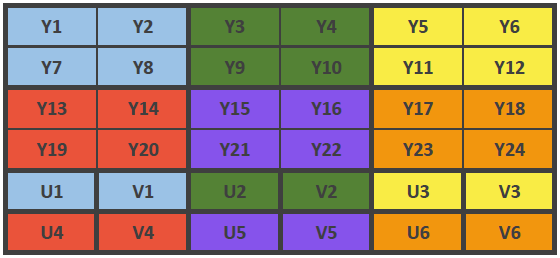
\includegraphics[width=0.5\textwidth]{Bilder/Materialien_und_Grundlagen/YUV_Frame.PNG}
	\caption{Frame im NV21-Format (YUV-Farbmodell)}
	\label{fig:YUV_Frame}
\end{figure}

~\\
Wie man unschwer erkennen kann, befinden sich die Informationen bezüglich der Luminanz in den ersten zwei Dritteln des Frames. Um aus einem Frame im YUV-Format ein Schwarzweißbild zu erzeugen, bräuchte man entsprechend nur diese Komponenten. 
\\
\\
Überführt man ein oben gezeigtes Frame (\ref{fig:YUV_Frame}) in ein eindimensionales Array, erhält man entsprechend folgende Aufteilung: 

\begin{figure}[h]
	\centering
	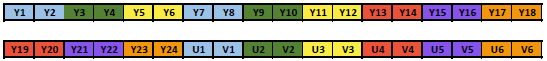
\includegraphics[width=1\textwidth]{Bilder/Materialien_und_Grundlagen/YUV_Array.PNG}
	\caption{Eindimensionales Array entsprechend eines Frames im NV21-Format (YUV-Farbmodell)}
	\label{fig:YUV_Array}
\end{figure}

\section{RGB-Farbmodell und Konvertierung} \label{YUV_RGBKonvert}

Das RGB-Farbmodell ist ein additives Farbmodell, bei dem die Farben durch Mischung der Grundfarben Rot, Grün und Blau dargestellt werden. Ein digitales Farbbild besitzt dabei für jeden Bildpunkt drei Werte, die die Anteile an Rot, Grün und Blau beschreiben. Der Wertebereich erstreckt sich dabei üblicherweise zwischen 0 und 255. Man kann sich dies als drei M x N Matrizen vorstellen: pro Grundfarbe eine Matrix, in der für jeden Pixel der Anteil der entsprechenden Grundfarbe gespeichert ist (siehe Abbildung \ref{fig:RGB-Matrizen}). \footcite{MTI2}


\begin{figure}[h]
	\centering
	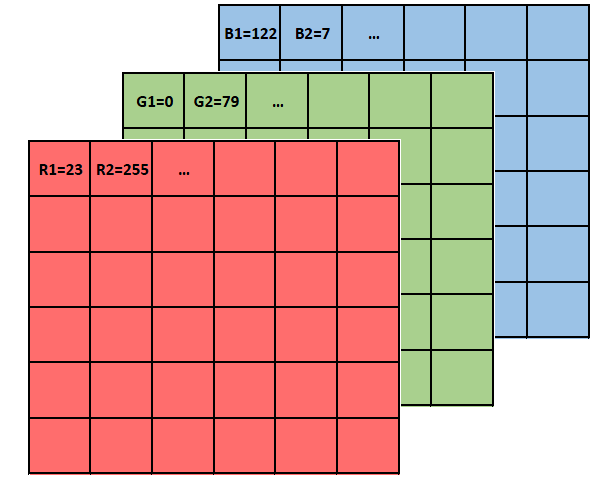
\includegraphics[width=0.55\textwidth]{Bilder/Materialien_und_Grundlagen/RGB_Matritzen2.png}
	\caption{Farbmatrizen des RGB-Farbmodells}
	\label{fig:RGB-Matrizen}
\end{figure}

Um die RGB-Werte eines Pixels aus einem Frame im YUV-Format zu ermitteln, müssen die entsprechenden Luminanz- und Chrominanzwerte dieses Pixels aus dem YUV-Frame ermittelt und in RGB-Werte umgerechnet werden. Bei der Wahl der Formel zur Umrechnung vom YUV-Farbformat in ein RGB-Farbformat ist zu beachten in welchem exakten Format sich das Ausgangsframe befindet. Die Frames, die in dieser Arbeit konvertiert werden mussten, befanden sich im Format YUV420, weshalb sich folgende Konstanten für die Umrechnungsformeln für die einzelnen Werte R, G und B eines Pixels ergaben \footcite{Konvertierung}:
\\

$R = clamp(Y + 1.402 \times V) $\\
$G = clamp(Y - 0.344 \times U - 0.714 \times V) $\\
$B = clamp(Y + 1.772 \times U) $\\